% Drawing 107/01-1 -- folder 107, batch 01, archive page 14 (PDF page 15).
% Transcription: à droite, un petit triangle hachuré, chacun des trois côtés marqué « $x_1$ ».
% Kind: hatched triangle with labelled sides. Method 2 (schematic redraw from the facsimile). Status: ok.
% Notes: A small triangle of three separate strokes that do not meet (the upper left one hooked at its foot), hatched with seven oblique strokes roughly parallel to the upper left side, one of them running out below the base; a small dot just outside each corner; the label x_1 beside each of the three sides. The label is read x_1 after the transcription; the letter could also be a y. The triple stroke joining X_{n-2} to X_{n-1} lower on the page, named in the same note, is a triple arrow, a relation to be set as text, and is not part of this drawing. Redrawn 2026-11-12 (issue 128): to check again. Question settled by a machine pass on the facsimile, 2026-11-12 (maths): the labels are x_1: the page works with a simplicial object X, whose 1-simplices x_1 are the sides of the triangle, and no y occurs on it. Not checked by a reader. Overlaid 2026-11-12 (Opus 5.5) on a 400 dpi colour render: the earlier redraw closed the triangle on computed vertices, its top corner some 3 units left of where the right stroke starts, and filled it with regular hatching; the three strokes, the seven hatching strokes, the three corner dots and the left label are now placed as on the page.
% Coordinates: 1 unit = 1 mm = 1/100 of the crop width (bbox in page fractions: [0.76, 0.19, 0.9, 0.27]).
% Redrawn by Claude (claude-fable-5-2), issue #128, 2026-11-12; not checked by a human; not compiled (no TeX in the session).
% Overlaid by Claude (claude-opus-5-5) 2026-11-12 (issue #128): rasterised from its own coordinates over the colour facsimile and checked or corrected. Not compiled. Status: ok.
% Rights: reproduces part of the work -- behind RENDER_TRANSCRIPTS, never published by itself.
\documentclass[tikz,border=3pt]{standalone}
\usepackage{amsmath,amssymb}
\usetikzlibrary{patterns,arrows.meta}
\tikzset{pencil/.style={black!45}, struck/.style={black!35}, mpt/.style={circle,draw,inner sep=1.3pt}, pt/.style={circle,fill,inner sep=0.9pt}, opt/.style={circle,draw,fill=white,inner sep=1.1pt}}
\begin{document}
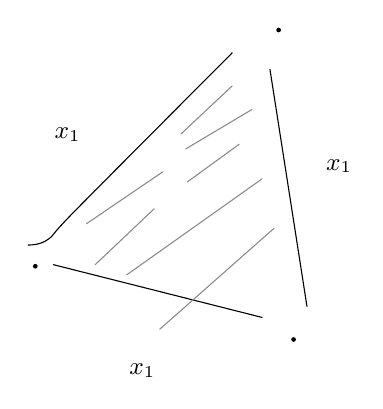
\begin{tikzpicture}[x=1mm,y=1mm,line cap=round,line join=round,font=\scriptsize]
\draw plot[smooth, tension=0.6] coordinates {(25.5,-49) (28,-48.3) (31.7,-44.4) (51.4,-24.6)};
\draw (56.2,-26.7) -- (60.9,-56.8);
\draw (28.7,-51.5) -- (55.2,-58.2);
\foreach \p in {(26.4,-51.7),(57.3,-21.7),(59.2,-61)} \node[pt,inner sep=0.6pt] at \p {};
\draw[pencil] (44.9,-34.9) -- (51.4,-28.8);
\draw[pencil] (45.5,-36.8) -- (53.9,-31.8);
\draw[pencil] (45.7,-41) -- (52.3,-36.2);
\draw[pencil] (32.9,-46.3) -- (42.6,-39.7);
\draw[pencil] (34,-51.5) -- (41.5,-44.4);
\draw[pencil] (38,-52.8) -- (55.2,-40.6);
\draw[pencil] (42.2,-59.7) -- (56.7,-46.9);
\node[inner sep=1pt] at (30.5,-35) {\small $x_1$};
\node[inner sep=1pt] at (65,-39) {\small $x_1$};
\node[inner sep=1pt] at (40,-65) {\small $x_1$};
\end{tikzpicture}
\end{document}
